\subsection{Decentralized SGF FW Experiments}
To study the performance of Algorithm \ref{decentralized} we split the 10000 images of the MNIST test set by giving 10 samples of each class to our 10 workers.
We then tuned the hyperparameter $m$, which identifies the directions of the additional noise, to find out the best value for which the lowest accuracy was reached.
\begin{figure}[htbp]
	\centering
	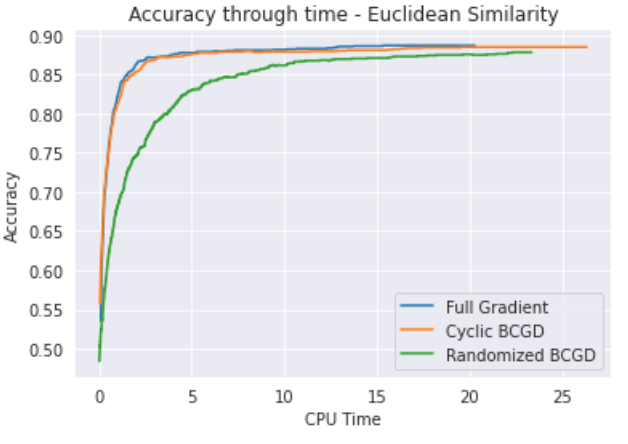
\includegraphics[width=6cm]{accuracy.png}
	\caption{{\small Accuracy of Algorithm \ref{decentralized} with respect to the change on the parameter m.}}
	\label{fig:accuracy}
\end{figure}
In Figure \ref{fig:accuracy} we can see a plot in which we represent the behaviour of the Decentralized SGF FW algorithm  with respect to the change of the parameter $m$. In particular, we can see that for $m=35$ the algorithm reaches an accuracy of approximately 20\%. With the increasing of $m$, the running time became very large and for this reason we had to find a value for $m$ which returns a low accuracy with respect to a reasonable running time. We ended up with $m=15$, which is a good balance between the two.\\
For our experiments we then fix $m=15$ and for each image we estimated its gradient using 20, 50 and 100 queries.

\begin{figure}[h]
	\centering
	\begin{subfigure}[b]{0.15\textwidth}
		\centering
		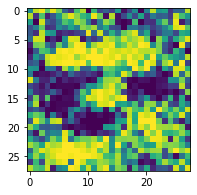
\includegraphics[width=2.3cm]{T20_final.png}
		\caption{}
		\label{fig:decentralized_perturbation_20}
	\end{subfigure}
	\hfill
	\begin{subfigure}[b]{0.15\textwidth}
		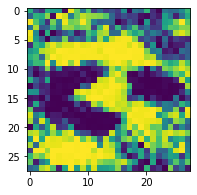
\includegraphics[width=2.3cm]{T50_final.png}
		\caption{}
		\label{fig:decentralized_perturbation_50}
	\end{subfigure}
	\hfill
	\begin{subfigure}[b]{0.15\textwidth}
		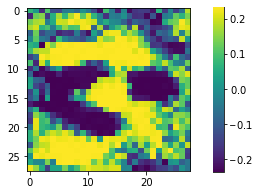
\includegraphics[width=3cm]{T100_bar.png}
		\caption{}
		\label{fig:decentralized_perturbation_100}
	\end{subfigure}
	\caption{{\small Perturbations of the Decentralized SGF FW algorithm with m=15: \ref{fig:decentralized_perturbation_20} for T=20, \ref{fig:decentralized_perturbation_50} for T=50,  \ref{fig:decentralized_perturbation_100} for T=100.}}
	\label{fig:decentralized_perturbations}
\end{figure}

As the number of queries increases, the pattern of the perturbation becomes clearer, and in Figure \ref{fig:decentralized_perturbations} we can see how the 3 becomes more defined as passing through the three queries. This phenomenon is due to the minimization of the respectively accuracy, that we reported in Table \ref{tab:decentralized}: to a lower accuracy corresponds a clearer pattern on the noise. It is interesting to notice that with just 20 queries the accuracy decrease to 55,25\% and so the digit images will be misclassified after 20 iterations. In Figure \ref{fig:decentralized} we can see the perturbation \ref{fig:decentralized_perturbation_100} applied on the digit of Class 4, labeled as a 3.

\begin{figure}[htbp]
	\centering
	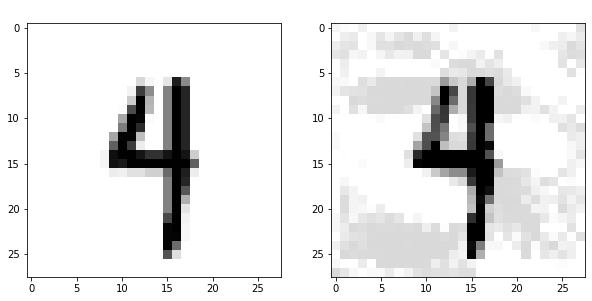
\includegraphics[width=7cm]{image_pertub_T100_final.png}
	\caption{{\small Image of 4 changed to 3 using the best adversarial perturbation generated by Algorithm \ref{decentralized} using perturbation \ref{fig:decentralized_perturbation_100}.}}
	\label{fig:decentralized}
\end{figure}

We made a comparison with a perturbation due to the gaussian noise in which the prediction is still very precise, with an accuracy of about 90\%. Even though the perturbation is not imperceptible, as we can see in Figure \ref{fig:gaussian_noise}, the network still classify correctly the images.

\begin{figure}[htbp]
	\centering
	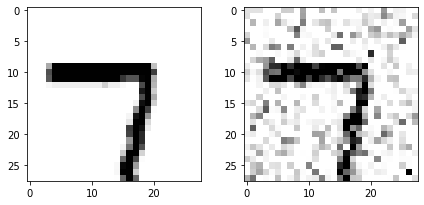
\includegraphics[width=7.25cm]{gaussian_image.png}
	\caption{{\small Gaussian perturbation on the original digit of a 7, still classify as a 7.}}
	\label{fig:gaussian_noise}
\end{figure}

\begin{table}[htbp]
	\begin{center}
		\begin{adjustwidth}{-.6cm}{}
			\begin{tabular}{c|ccc}
				\textbf{Attack} &          20 \textbf{queries} &      50 \textbf{queries} &     100 \textbf{queries} \\
				\midrule
				{\small Decentralized SGF FW}     &    55,25\% &    39,46\% &       36,87\% \\
			\end{tabular}
		\end{adjustwidth}
	\end{center}
	\caption{{\small Summary of $\ell_\infty$ Universal Adversarial Perturbation with $\varepsilon$=0.25. MNIST attack using Decentralized SGF FW. The number of queries in the column denote the number of queries used per image.}}
	\label{tab:decentralized}
\end{table}

It is noteworthy the comparison between the two type of perturbations analysed: the one from the Decentralized SGF FW and the one from the Gaussian noise. The former is characterize by a noise with a clear pattern that covers the majority of the image space while the other spread the noise randomly in the space, and due to the different characteristics, the Decentralized perturbations are able to fool the network on most images.